%%%%%%%%%%%%%%%%%%%%%%%%%%%%%%%%%%%%%%%%
% datoteka diploma-vzorec.tex
%
% vzorčna datoteka za pisanje diplomskega dela v formatu LaTeX
% na UL Fakulteti za računalništvo in informatiko
%
% vkup spravil Gašper Fijavž, december 2010
% 
%
%
% verzija 12. februar 2014 (besedilo teme, seznam kratic, popravki Gašper Fijavž)
% verzija 10. marec 2014 (redakcijski popravki Zoran Bosnić)
% verzija 11. marec 2014 (redakcijski popravki Gašper Fijavž)
% verzija 15. april 2014 (pdf/a 1b compliance, not really - just claiming, Damjan Cvetan, Gašper Fijavž)
% verzija 23. april 2014 (privzeto cc licenca)
% verzija 16. september 2014 (odmiki strain od roba)
% verzija 28. oktober 2014 (odstranil vpisno številko)
% verija 5. februar 2015 (Literatura v kazalu, online literatura)
% verzija 25. september 2015 (angl. naslov v izjavi o avtorstvu)
% verzija 26. februar 2016 (UL izjava o avtorstvu)
% verzija 16. april 2016 (odstranjena izjava o avtorstvu)
% verzija 5. junij 2016 (Franc Solina dodal vrstice, ki jih je označil s svojim imenom)


\documentclass[a4paper, 12pt]{book}
%\documentclass[a4paper, 12pt, draft]{book}  Nalogo preverite tudi z opcijo draft, ki vam bo pokazala, katere vrstice so predolge!



\usepackage[utf8x]{inputenc}   % omogoča uporabo slovenskih črk kodiranih v formatu UTF-8
\usepackage[slovene,english]{babel}    % naloži, med drugim, slovenske delilne vzorce
\usepackage[pdftex]{graphicx}  % omogoča vlaganje slik različnih formatov
\usepackage{fancyhdr}          % poskrbi, na primer, za glave stranif
\usepackage{amssymb}           % dodatni simboli
\usepackage{amsmath}           % eqref, npr.
%\usepackage{hyperxmp}
\usepackage[hyphens]{url}  % dodal Solina
\usepackage{comment}       % dodal Solina

\usepackage[pdftex, colorlinks=true,
						citecolor=black, filecolor=black, 
						linkcolor=black, urlcolor=black,
						pagebackref=false, 
						pdfproducer={LaTeX}, pdfcreator={LaTeX}, hidelinks]{hyperref}

\usepackage{color}       % dodal Solina
\usepackage{soul}       % dodal Solina

%%%%%%%%%%%%%%%%%%%%%%%%%%%%%%%%%%%%%%%%
%	DIPLOMA INFO
%%%%%%%%%%%%%%%%%%%%%%%%%%%%%%%%%%%%%%%%
\newcommand{\ttitle}{Elektronsko naročanje v restavraciji}
\newcommand{\ttitleEn}{Diploma thesis sample}
\newcommand{\tsubject}{\ttitle}
\newcommand{\tsubjectEn}{\ttitleEn}
\newcommand{\tauthor}{Luka Horvat}
\newcommand{\tkeywords}{Slovenija, naročanje, neuspešni projekti, rešitev, spletna aplikacija}
\newcommand{\tkeywordsEn}{computer, computer, computer}


%%%%%%%%%%%%%%%%%%%%%%%%%%%%%%%%%%%%%%%%
%	HYPERREF SETUP
%%%%%%%%%%%%%%%%%%%%%%%%%%%%%%%%%%%%%%%%
\hypersetup{pdftitle={\ttitle}}
\hypersetup{pdfsubject=\ttitleEn}
\hypersetup{pdfauthor={\tauthor, matjaz.kralj@fri.uni-lj.si}}
\hypersetup{pdfkeywords=\tkeywordsEn}


 


%%%%%%%%%%%%%%%%%%%%%%%%%%%%%%%%%%%%%%%%
% postavitev strani
%%%%%%%%%%%%%%%%%%%%%%%%%%%%%%%%%%%%%%%%  

\addtolength{\marginparwidth}{-20pt} % robovi za tisk
\addtolength{\oddsidemargin}{40pt}
\addtolength{\evensidemargin}{-40pt}

\renewcommand{\baselinestretch}{1.3} % ustrezen razmik med vrsticami
\setlength{\headheight}{15pt}        % potreben prostor na vrhu
\renewcommand{\chaptermark}[1]%
{\markboth{\MakeUppercase{\thechapter.\ #1}}{}} \renewcommand{\sectionmark}[1]%
{\markright{\MakeUppercase{\thesection.\ #1}}} \renewcommand{\headrulewidth}{0.5pt} \renewcommand{\footrulewidth}{0pt}
\fancyhf{}
\fancyhead[LE,RO]{\sl \thepage} 
%\fancyhead[LO]{\sl \rightmark} \fancyhead[RE]{\sl \leftmark}
\fancyhead[RE]{\sc \tauthor}              % dodal Solina
\fancyhead[LO]{\sc Diplomska naloga}     % dodal Solina


\newcommand{\BibTeX}{{\sc Bib}\TeX}

%%%%%%%%%%%%%%%%%%%%%%%%%%%%%%%%%%%%%%%%
% naslovi
%%%%%%%%%%%%%%%%%%%%%%%%%%%%%%%%%%%%%%%%  


\newcommand{\autfont}{\Large}
\newcommand{\titfont}{\LARGE\bf}
\newcommand{\clearemptydoublepage}{\newpage{\pagestyle{empty}\cleardoublepage}}
\setcounter{tocdepth}{2}	      % globina kazala

%%%%%%%%%%%%%%%%%%%%%%%%%%%%%%%%%%%%%%%%
% konstrukti
%%%%%%%%%%%%%%%%%%%%%%%%%%%%%%%%%%%%%%%%  
\newtheorem{izrek}{Izrek}[chapter]
\newtheorem{trditev}{Trditev}[izrek]
\newenvironment{dokaz}{\emph{Dokaz.}\ }{\hspace{\fill}{$\Box$}}

%%%%%%%%%%%%%%%%%%%%%%%%%%%%%%%%%%%%%%%%%%%%%%%%%%%%%%%%%%%%%%%%%%%%%%%%%%%%%%%
%% PDF-A
%%%%%%%%%%%%%%%%%%%%%%%%%%%%%%%%%%%%%%%%%%%%%%%%%%%%%%%%%%%%%%%%%%%%%%%%%%%%%%%


%%%%%%%%%%%%%%%%%%%%%%%%%%%%%%%%%%%%%%%% 
% define medatata
%%%%%%%%%%%%%%%%%%%%%%%%%%%%%%%%%%%%%%%% 
\def\Title{\ttitle}
\def\Author{\tauthor, matjaz.kralj@fri.uni-lj.si}
\def\Subject{\ttitleEn}
\def\Keywords{\tkeywordsEn}

%%%%%%%%%%%%%%%%%%%%%%%%%%%%%%%%%%%%%%%% 
% \convertDate converts D:20080419103507+02'00' to 2008-04-19T10:35:07+02:00
%%%%%%%%%%%%%%%%%%%%%%%%%%%%%%%%%%%%%%%% 
\def\convertDate{%
    \getYear
}

{\catcode`\D=12
 \gdef\getYear D:#1#2#3#4{\edef\xYear{#1#2#3#4}\getMonth}
}
\def\getMonth#1#2{\edef\xMonth{#1#2}\getDay}
\def\getDay#1#2{\edef\xDay{#1#2}\getHour}
\def\getHour#1#2{\edef\xHour{#1#2}\getMin}
\def\getMin#1#2{\edef\xMin{#1#2}\getSec}
\def\getSec#1#2{\edef\xSec{#1#2}\getTZh}
\def\getTZh +#1#2{\edef\xTZh{#1#2}\getTZm}
\def\getTZm '#1#2'{%
    \edef\xTZm{#1#2}%
    \edef\convDate{\xYear-\xMonth-\xDay T\xHour:\xMin:\xSec+\xTZh:\xTZm}%
}

\expandafter\convertDate\pdfcreationdate 

%%%%%%%%%%%%%%%%%%%%%%%%%%%%%%%%%%%%%%%%
% get pdftex version string
%%%%%%%%%%%%%%%%%%%%%%%%%%%%%%%%%%%%%%%% 
\newcount\countA
\countA=\pdftexversion
\advance \countA by -100
\def\pdftexVersionStr{pdfTeX-1.\the\countA.\pdftexrevision}


%%%%%%%%%%%%%%%%%%%%%%%%%%%%%%%%%%%%%%%%
% XMP data
%%%%%%%%%%%%%%%%%%%%%%%%%%%%%%%%%%%%%%%%  
\usepackage{xmpincl}
\includexmp{pdfa-1b}

%%%%%%%%%%%%%%%%%%%%%%%%%%%%%%%%%%%%%%%%
% pdfInfo
%%%%%%%%%%%%%%%%%%%%%%%%%%%%%%%%%%%%%%%%  
\pdfinfo{%
    /Title    (\ttitle)
    /Author   (\tauthor, damjan@cvetan.si)
    /Subject  (\ttitleEn)
    /Keywords (\tkeywordsEn)
    /ModDate  (\pdfcreationdate)
    /Trapped  /False
}


%%%%%%%%%%%%%%%%%%%%%%%%%%%%%%%%%%%%%%%%%%%%%%%%%%%%%%%%%%%%%%%%%%%%%%%%%%%%%%%
%%%%%%%%%%%%%%%%%%%%%%%%%%%%%%%%%%%%%%%%%%%%%%%%%%%%%%%%%%%%%%%%%%%%%%%%%%%%%%%

\begin{document}
\selectlanguage{slovene}
\frontmatter
\setcounter{page}{1} %
\renewcommand{\thepage}{}       % preprecimo težave s številkami strani v kazalu
\newcommand{\sn}[1]{"`#1"'}                    % dodal Solina (slovenski narekovaji)

%%%%%%%%%%%%%%%%%%%%%%%%%%%%%%%%%%%%%%%%
%naslovnica
 \thispagestyle{empty}%
   \begin{center}
    {\large\sc Univerza v Ljubljani\\%
      Fakulteta za računalništvo in informatiko}%
    \vskip 10em%
    {\autfont \tauthor\par}%
    {\titfont \ttitle \par}%
    {\vskip 3em \textsc{DIPLOMSKO DELO\\[5mm]         % dodal Solina za ostale študijske programe
%    VISOKOŠOLSKI STROKOVNI ŠTUDIJSKI PROGRAM\\ PRVE STOPNJE\\ RAČUNALNIŠTVO IN INFORMATIKA}\par}%
    VISOKOŠOLSKI ŠTUDIJSKI PROGRAM \\ PRVE STOPNJE\\ RAČUNALNIŠTVO IN INFORMATIKA}\par}%
%    INTERDISCIPLINARNI UNIVERZITETNI\\ ŠTUDIJSKI PROGRAM PRVE STOPNJE\\ RAČUNALNIŠTVO IN MATEMATIKA}\par}%
%    INTERDISCIPLINARNI UNIVERZITETNI\\ ŠTUDIJSKI PROGRAM PRVE STOPNJE\\ UPRAVNA INFORMATIKA}\par}%
%    INTERDISCIPLINARNI UNIVERZITETNI\\ ŠTUDIJSKI PROGRAM PRVE STOPNJE\\ MULTIMEDIJA}\par}%
    \vfill\null%
    {\large \textsc{Mentorica}: doc. dr. Mira Trebar\par}%
   {\large \textsc{Somentor}: as. dr. David Jelenc \par}%
    {\vskip 2em \large Ljubljana, 2021 \par}%
\end{center}
% prazna stran
%\clearemptydoublepage      % dodal Solina (izjava o licencah itd. se izpiše na hrbtni strani naslovnice)

%%%%%%%%%%%%%%%%%%%%%%%%%%%%%%%%%%%%%%%%
%copyright stran
\thispagestyle{empty}
\vspace*{8cm}

\noindent
{\sc Copyright}. 
Rezultati diplomske naloge so intelektualna lastnina avtorja in Fakultete za računalništvo in informatiko Univerze v Ljubljani.
Za objavo in koriščenje rezultatov diplomske naloge je potrebno pisno privoljenje avtorja, Fakultete za računalništvo in informatiko ter mentorja.

\begin{center}
\mbox{}\vfill
\emph{Besedilo je oblikovano z urejevalnikom besedil \LaTeX.}
\end{center}
% prazna stran
\clearemptydoublepage

%%%%%%%%%%%%%%%%%%%%%%%%%%%%%%%%%%%%%%%%
% stran 3 med uvodnimi listi
\thispagestyle{empty}
\vspace*{4cm}

\noindent
Fakulteta za računalništvo in informatiko izdaja naslednjo nalogo:
\medskip
\begin{tabbing}
\hspace{32mm}\= \hspace{6cm} \= \kill




Tematika naloge: Elektronsko naročanje v restavracij
\end{tabbing}
Besedilo teme diplomskega dela študent prepiše iz študijskega informacijskega sistema, kamor ga je vnesel mentor. V nekaj stavkih bo opisal, kaj pričakuje od kandidatovega diplomskega dela. Kaj so cilji, kakšne metode uporabiti, morda bo zapisal tudi ključno literaturo.
\vspace{15mm}






\vspace{2cm}

% prazna stran
\clearemptydoublepage

% zahvala
\thispagestyle{empty}\mbox{}\vfill\null\it%
\noindent
Na tem mestu zapišite, komu se zahvaljujete za izdelavo diplomske naloge. Pazite, da ne boste koga pozabili. Utegnil vam bo zameriti. Temu se da izogniti tako, da celotno zahvalo izpustite.
\rm\normalfont

% prazna stran
\clearemptydoublepage

%%%%%%%%%%%%%%%%%%%%%%%%%%%%%%%%%%%%%%%%
% posvetilo, če sama zahvala ne zadošča :-)
%\thispagestyle{empty}\mbox{}{\vskip0.20\textheight}\mbox{}\hfill\begin{minipage}{0.55\textwidth}%
%Svoji dragi Alenčici.
%\normalfont\end{minipage}

% prazna stran
\clearemptydoublepage


%%%%%%%%%%%%%%%%%%%%%%%%%%%%%%%%%%%%%%%%
% kazalo
\pagestyle{empty}
\def\thepage{}% preprecimo tezave s stevilkami strani v kazalu
\tableofcontents{}

% prazna stran
\clearemptydoublepage

%%%%%%%%%%%%%%%%%%%%%%%%%%%%%%%%%%%%%%%%
% seznam kratic

\chapter*{Seznam uporabljenih kratic}  % spremenil Solina, da predolge vrstice ne gredo preko desnega roba

\begin{comment}
\begin{tabular}{l|l|l}
  {\bf kratica} & {\bf angleško} & {\bf slovensko} \\ \hline
  % after \\: \hline or \cline{col1-col2} \cline{col3-col4} ...
  {\bf SPA} & single page application & aplikacija na eni strani \\
  {\bf SQL} & structured query language & strukturirani povpraševalni jezik za delo s podatkovnimi bazami  \\
  {\bf SVM} & support vector machine & metoda podpornih vektorjev \\
  {\bf SVM}   & support vector machine              & metoda podpornih vektorjev \\
  \dots & \dots & \dots \\
\end{tabular}
\end{comment}

\noindent\begin{tabular}{p{0.1\textwidth}|p{.4\textwidth}|p{.4\textwidth}}    % po potrebi razširi prvo kolono tabele na račun drugih dveh!
  {\bf kratica} & {\bf angleško}                             & {\bf slovensko} \\ \hline
  {\bf SPA}      & single page application               &  aplikacija na eni strani \\
  {\bf SQL} & structured query language & strukturirani povpraševalni jezik za delo s podatkovnimi bazami  \\
  {\bf CLI}   & command-line interface              & znakovni uporabniški vmesnik \\
%  \dots & \dots & \dots \\
\end{tabular}


% prazna stran
\clearemptydoublepage

%%%%%%%%%%%%%%%%%%%%%%%%%%%%%%%%%%%%%%%%
% povzetek
\addcontentsline{toc}{chapter}{Povzetek}
\chapter*{Povzetek}

\noindent\textbf{Naslov:} \ttitle
\bigskip

\noindent\textbf{Avtor:} \tauthor
\bigskip

%\noindent\textbf{Povzetek:} 
\noindent 
Slovenija velja za državo z veliko število restavracij, vendar le malo iz med njih uporablja napredne sisteme naročanja kot npr. ena izmed večjih verig s hitro prehrano, McDonalds. V Sloveniji je bilo nekaj projektov s podobnimi idejami, vendar z napačnimi cilji zaradi katerih so bili neuspešni. Eden izmed razlogov, da jim ni uspelo, je bilo sabotiranje sistemov s strani natakarjev, saj so misli da bo tehnologija zamenjala njegove službe. V zavedanju teh problematik smo se odločil narediti diplomski nalogo na to temo. Rezultat je aplikacija katero lahko uporabimo kot pregledovalnik hrane in pijače, ki jo ponuja restavracija, ali pa kot sistem za naročanje. Njen glavni namen je olajšati delo natakarjem in kuharjem. S tem bi pridobili na času, kar bi izbošljšalo kvaliteto in hitrost postrežbe ter izdelave hrane in pijače. 
V diplomski nalogi najprej opišemo kako smo prišli do ideje, sam razvoj in delovanje aplikacije. Na koncu smo naredili tudi primerjavo s trenutno konkurenco na trgu oziroma z aplikacijo, ki vemo da ni uspela. 

\noindent\textbf{Ključne besede:} \tkeywords.
% prazna stran
\clearemptydoublepage

%%%%%%%%%%%%%%%%%%%%%%%%%%%%%%%%%%%%%%%%
% abstract
\selectlanguage{english}
\addcontentsline{toc}{chapter}{Abstract}
\chapter*{Abstract}

\noindent\textbf{Title:} \ttitleEn
\bigskip

\noindent\textbf{Author:} \tauthor
\bigskip

%\noindent\textbf{Abstract:} 
\noindent This sample document presents an approach to typesetting your BSc thesis using \LaTeX. 
A proper abstract should contain around 100 words which makes this one way too short.
\bigskip

\noindent\textbf{Keywords:} \tkeywordsEn.
\selectlanguage{slovene}
% prazna stran
\clearemptydoublepage

%%%%%%%%%%%%%%%%%%%%%%%%%%%%%%%%%%%%%%%%
\mainmatter
\setcounter{page}{1}
\pagestyle{fancy}

\chapter{Uvod}
Tehnologije v sedanjem času predstavljajo velik napredek na vseh področij. Na strani gostinstva ni drastičnih napredkov, saj sem to ugotovil kar na osnovi lastnih izkušen. Kot študent fakultete za računalništvo in informatiko sem opravljal delo v eni izmed restavracij, saj biti študent z dodatnim zaslužkom ni dilema. Opravljal sem delo dostavljavca hrane v eni izmed bližnji restavraciji, hkrati pa opazoval potek dela v kuhinji in strežbi. Kasneje sem napredoval v strežbo in kot programer hitro opazil stvari, ki bi se jih dalo izboljšati. Najbolj me je motilo nezadovoljstvo strank ob veliki zasedenosti restavracije. Preprosto en človek ne uspe postreči več kot eno mizo na enkrat. Zato sem si zamislil sistem za naročanje hrane, ki ne bi bil namenjen zamenjavi ljudi v strežbi, vendar kot pregledovalnik (angl. Menu) ali pa kot sistem za naročanju hrane in pijače. Stranka bi bila tista, ki bi se odločila ali želi pri naročanju uporabiti stik z osebo v strežbi ali bi preprosto naročila z uporabo aplikacije na tablici, ki bi bila vedno dosegljiva na vsaki mizi. 
\section {Problematika}
Z izdelavo spletne aplikacije sem želel zagotoviti lažje delovanje restavracij predvsem olajšati delo natakarjem, ki bi se potem lažje osredotočili na kakovost postrežbe pijač in jedi. Izboljšati sem želel čas postrežbe gostov, kar bi prizaneslo tudi k večjemu število postreženih gostov v nekem časovnem obdobju. Naredil sem analizo, ki si jo lahko pogledate v članku 3.2. Vsekakor ni moja aplikacija namenjena zamenjavi delovnih mest, vendar samo pohitritvi strežbe. To bi vplivalo tudi na zmanjšanje časa, ki ga gost porabi v primeru, da je natakar zelo zaseden. Obstajajo tablice, katere uporabljajo natakarji pri sprejemanju naročil, ki predvsem pomagajo, da si ne rabijo vsega zapomniti in da lahko pobirajo zaporedna naročila. Iz lastnih izkušenj vem, da z uporabo spomina pride hitreje do napak, saj si preprosto ne moreš vsega zapomniti. Težava je tudi v tem, da moraš za vsako pobrano naročilo do blagajne, da naročilo ne čaka in čimprej pride do kuharja oziroma natakarja, ki pripravlja pijače. Po navadi največ pri pobiranju naročil vzamejo  gosti, ki se radi premišljujejo zadnje minute, kar ni nič narobe. Ko sem opravljal delo natakarja sem se spraševal zakaj ne bi ta čas raje posvetil strežbi oziroma pripravi naročil, kot pa pobiranju naročil strank, ki ne vedo kaj bi. Ta aplikacija bi še dodatno zmanjšala čas pobiranja naročil, saj natakar včasih pride prehitro ali pa prepozno, vendar z uporabo aplikacije bi bilo naročanje vedno na voljo. 

\section {Ideja}
Aplikacijo sem si zamislil v treh pogledih, in sicer uporabnik oziroma gost, natakar in kuhar. Gost bi imel na voljo pregled vseh pijač in jedi, ki jih restavracija ponuja. S tem bi pripomogel k ekologiji, saj restavracije ne bi več potrebovale papirnatih menijev. Natakar in kuhar bi imela pregled nad naročili. Naročilo bi razdelil v dva dela, da ima tako natakar kot kuhar nadzor samo nad svojimi naročili. S tem bi omogočil, da se lahko kreira statistika za vsakega posebej.

\chapter{Uporabljene tehnologije in programske opreme}
V diplomski nalogi sem se srečeval predvsem z naslednjimi programskimi jeziki: JavaScript, Python, SQL. Vse podrobnosti pa so opisane v spodnjih poglavjih.

\section {Vue.js}
JavaScript je programski jezik, zaradi katerega so spletne strani postale dinamične in bolj zmogljive. Z njem smo programsko kodo, ki je bila na strežniškem delu, preselili v brskalnik. Tako smo na začetku dobili veliko JavaScript programske kode povezane z različnimi HTML in CSS datotekami brez kakršne koli formalne organizacije (poznano kot «script»). Zaradi tega smo razvijalci začeli uporabljati JavaScript Frameworks, saj poenostavijo izdelavo aplikacij.


Vue je eden izmed mnogih kot npr. Angular, Ember, React,… poznan pa je predvsem zaradi enostavnosti za upravljanje in izvajanje testov. Vsem je skupna točka reaktivnost, vendar v drugačnem pomenu besede. Gre za to, da se aplikacija postopno prilagaja glede na vrednosti podatkov. 


\subsection {Kaj je reaktivnost?}
Reaktivnost \cite{reaktivnost}, je programska paradigma, ki nam omogoča, da se na deklarativni način prilagodimo spremembam. Dober primer reaktivnosti je npr. funkcija SUM, ki jo uporabljamo v Excelu. Slika~\ref{Excel-SUM} prikazuje primer v Excelu.
\begin{figure}[h]
\begin{center}
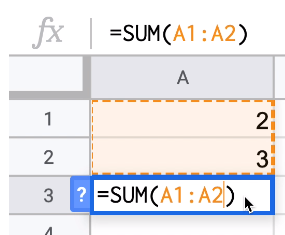
\includegraphics[width=7cm]{Excel-SUM.png}
\end{center}
\caption{Primer fukcije SUM v programu Excel}
\label{Excel-SUM}
\end{figure}

Če vstavimo številko 2 v prvo celico in številko 3 v drugo celico ter izberemo funkcijo SUM teh dveh celic. Kot rezultat dobimo vsoto obeh številk skupaj, kar ni nič posebnega. Vendar če bomo spremenili vrednost prve celice, bo funkcija SUM avtomatsko posodobila skupno vrednost. Tako deluje tudi reaktivnost v aplikacijah za razliko, da je podatek lahko vezan na več funkciji oziroma delov programske kode, ki se ob spremembi vrednosti posodobijo.

\subsection {Delovanje reaktivnost v Vue}
Vue se torej v primerjavi z navadnim JavaScriptom sprehodi skozi podatke in njihove lastnosti (angl. Properties) pretvori v fukciji Getter in Setter, ki sta nevidni uporabniku \cite{delovanjeReaktivnost}. Poglejte si sliko~\ref{VueReacitivity} za lažjo predstavo. 

Torej funkcija Getter pokliče instanco Watcher z namenom odvisnosti do drugih komponent. To pomeni, če je podatek označen kot odvisen (angl.  Dependency) bodo nekateri deli programske kode oziroma funkcije poklicane vsakič, ko se spremeni vrednost podatka. Funkcija Setter pa obvesti instanco Watcher, vsakič ko se podatku spremeni lastnost. Ta poskrbi, da se pokliče funkcija upodabljanja (angl. Render) tiste komponente, ki potem prikaže spremembe v samem pogledu aplikacije. 

\begin{figure}[h]
\begin{center}
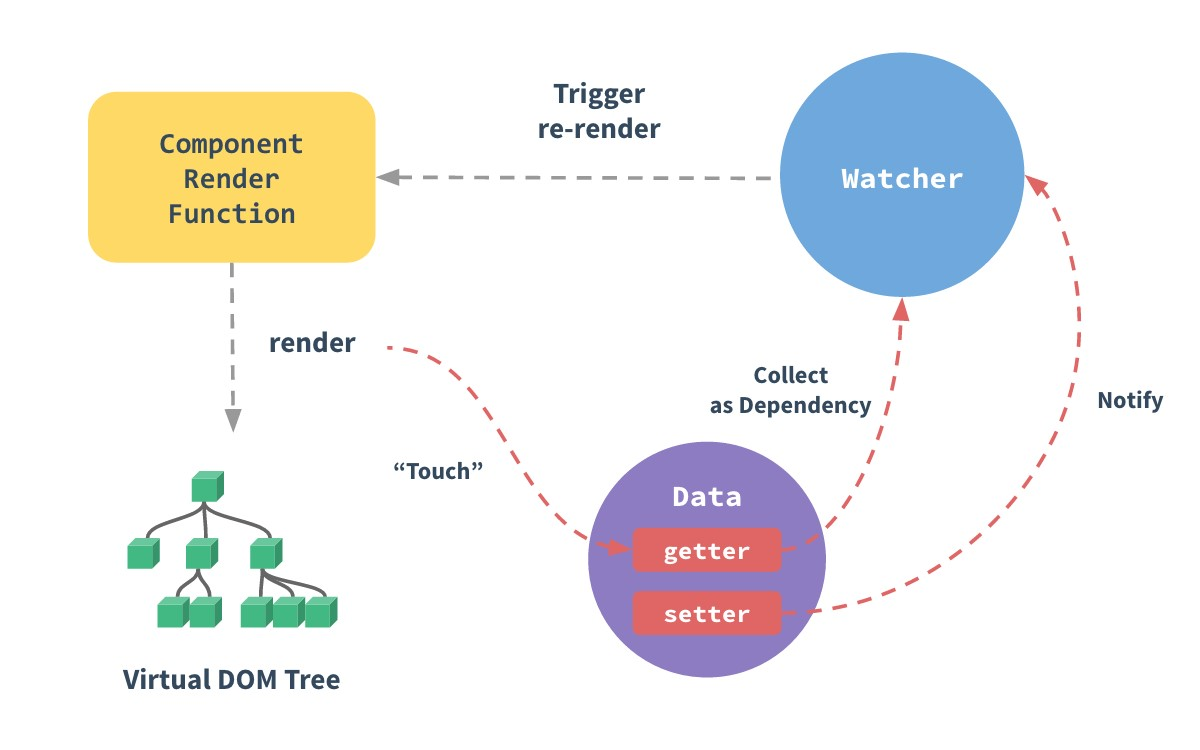
\includegraphics[width=13cm]{Vue-reactivity.jpg}
\end{center}
\caption{Kateri dialekt uporabljati?}
\label{VueReacitivity}
\end{figure}

\subsection {Knjižnice in dodatki}

Tako kot vsak programski jezik ima tudi Vue svoje dodatke, ki pomagajo pri razvoju aplikaciji. Spodnje sem uporabljal sam in so vredni omembe.
\begin{description}
\item[Vue CLI] velja kot standardno orodje za ekosistem Vue \cite{VueCLI}. Zagotavlja, da že pri gradnji novega projekta poveže različne dodatke med seboj. To omogoča razviljacu, da se bolj osredotoči na programiranje in ne na povezovanje njih v projekt. Zadeva izgleda nekako tako, da preko CLI vmesnika izbereš kakšen projekt želiš. Imaš seveda že privzete nastavitve, vendar omogoča tudi nastavljanje po meri. Sam sem uporabil Vuex, Vue-Router, ESLint in Vuetify.
\item[Vuex] je knjižnica za shranjevanje vrednosti v aplikacijah Vue.js \cite{Vuex}. Služi kot centralizirana baza podatkov za vse komponente v aplikaciji. 
\item[Vue-Router] je uradni usmerjevalnik za Vue.js \cite{VueRouter}. Integrira se globoko z jedrom Vue.js, tako da poenostavi izdelavo SPA aplikacij. Usmerjevalki je mišljen v smislu usmerjanja na druge komponente (angl. Component), ki v Vue.js predstavljajo druge poglede, lahko bi rekli podobno kot podstrani.
\item[ESLint] je orodje za prepoznavanje in poročanje o popravkih v programski kodi \cite{ESLint}. Cilje je narediti kodo bolj pregledno in urejeno, kar pripomore k izogibanju napak.
\item[Vuetify] je eden izmed mnogih uporabniških vmesnikov, ki je zgrajen na vrhu Vue.js \cite{Vuetify}. Za razliko od drugih vmesnikov je Vuetiy enostaven za učenje z več stotimi komponentami izdelanih po specifikacijah Material Design.
\item[Vue-devtools] je zgolj dodatek v brskalniku, ki omogoča lažje sledenje delovanja aplikacije in odpravljanju napak. 
\end{description}


\section {Python/Flask}
Flask je eno izmed najbolj popularnih spletno aplikacijskih vmesnikov (angl. Freamwork) \cite{Flask}. Zasnovan je tako, da omogoča hiter in enostaven začetek z možnostjo razširitve na zapletene aplikacije. V primerjavi z Django spletnim vmesnikov je za enak primer veliko bolj ekspliciten. Flask je prvotno zasnoval in razvil Armin Ronacher kot prvoaprilsko šalo leta 2010. Kljub taki predstavitvi je Flask postal izjemno priljubljen kot alternativa projektom narejenih v Django. Jaz sem ga uporabil za komunikacijo med aplikacijo in podatkovno bazo. Je enostaven za uporabo z veliko podpore na spletu. 

\section {MySQL/Toad DataModler}
MySQL je eden od odprtokodnih sistemov za upravljanje s podatkovni bazami, ki za delo s podatki uporablja jezik SQL. Napisan je v programskem jeziku C in C++ in deluje v vseh modernih sistemih npr. Windows, Linux, OS X,… Prva verzija je bil razvita leta 1995 s strani Michael Widenius in David Axmark. Kratica My izhaja iz imena prve hčerke očeta Michaela.  


Toad DataModler je orodje za izdelavo visokokakovostnih podatkovnih modelov. Omogoča izdelavo logičnih in fizičnih podatkovnih modelov, kar pripore k lažjem razumevanju in razvijanju podatkovne baze. Njegova najboljša funkcionalnost je, da lahko generiramo SQL kodo v različne podatkovne sisteme kot npr. MySQL, Ingres, Microsoft Azurem, Microsoft Access, Mircrosoft SQL Server,... Program sem uporabil prav zato, da sem najprej naredil fizični podatkovni model ter nato generiral MySQL kodo. 

\section {Viusal Studio}
Visual Studi Code je odprtokodno razvojno orodje, ki ga je razvil Microsoft leta 2015. Namenjeno je razvoju programov v operacijskem sistemu Windows. Omogoča razvoj aplikacij v jeziku C, C++, Python, Visual Basic .NET, JavaScript,… 

Orodje v osnovi omogoča veliko funkcionalnosti, npr. razhroščevanje, popravljanje sintaktičnih napak, avtomatično dopolnjevanje programske kode, izvajanje programske kode v realnem času, dostop do CLI vmesnika, povezavo z GIT,… Kar ni vključeno v orodje je mogoče dodati z razširitvami, ki se jih brezplačno namesti znotraj orodja. Sam sem si namestil razširitev za Vue.js s katerimi sem pridobil avtomatsko dopolnjevanje kode in ESLint, da se je nepravilno urejena koda sproti označevala.  

\section {XAMPP}
XAMPP je odprtokodni strežnik za razvoj spletnih aplikacij, ki se uporablja lokalno za testne projekte predno postanejo aktivni vsem preko spleta. Ta strežnik za razvoj spletnih aplikacij vsebuje tudi druge pred namestitvene aplikacije, kot so Apache spletni strežnik, MySQL podatkovno bazo, PHP in Perl. Deluje na vseh platformah Linux, Windows in Mac OS. Vse aplikacije se vklaplja preko XAMPP nadzorne plošče.


PhpMyAdmin je ime za spletni vmesnik, ki omogoča upravljane z MySQL podatkovnimi bazami. Program je vključen v XAMPP in sicer znotraj aplikacije MySQL. Je zelo močno orodje in predvsem enostavno za uporabo. Sam sem ga uporabil pri testiranju poizvedb in dodajanju podatkov v podatkovno bazo.

\section {GitHub}
GitHub je spletna platforma za distribuirano upravljanje s programsko kodo, ki je bila ustanovljena februarja leta 2008 \cite{GitHub}. Razvita je bil iz programa Git, ki je lokalna različica GitHuba. Njen poudarek je predvsem na hitrosti, integriteti podatkov in vzporednem toku dela. Namenjen je tako za samostojni kot tudi za kolaborantovi razvoj. Začneš tako, da ustvariš repozitoriji, ki predstavlja glavno programsko kodo. Iz tega se lahko naredi več podružnic (angl. Branch), ki predstavljajo kopijo glavne kode na kateri se lahko izvajajo testi oziroma odpravljajo težav. Podružnice potem združuješ in tako glavna programska koda ne vsebuje napak oziroma predstavlja vedno delujoč izdelek. 

Git Hub Desktop je aplikacija za operacijske sisteme, ki je zelo enostavna. Ponuja vse funkcionalnosti kot na spletu, vendar zaradi uporabe lokalnih orodij veliko bolj priročna. Ko zaključiš delo narediš Commit in Push ter vse spremembe shraniš v repozitoriji na spletu. Tako nikoli ne izgubiš projekta oziroma imaš sinhronizacijo z ostalimi ljudmi na projektu. 


\chapter {Struktura in razvoj aplikacije}

\section{Podatkovna baza}
Izdelavo podatkovne baze sem se lotil v programu Toad DataModler, slika~\ref{Database_physical}. Baza je sestavljena iz osmih tabel, katere sem bolj podrobno opisal spodaj. 

FoodType tabela je namenjana zapisom vrsti jedi t.i. predjedi, glavne jedi, sladice,… Sestavljena je iz atributov: ID, Name.

DrinkType tabela je namejna vrsti pijač, npr. sokovi, koktejli, piva, topli napitki,… Sestavljena je enakih atirbutov kot FoodType.

Food tabela je namenjena opisu hrane in je sestavljena iz atributov: ID, Name, Price, Size, Calorie, Picture in Description.  V atribut Picture se zapiše ime slike, ki se prikaže v aplikaciji. Vse slike sem hranil v datoteki na lokalnem strežniku Apache.

Drink tabela je namenjan opisu pijače in je sestavljena iz enakih atributov kot Food le da ima še enega dodatnega z imenom Alcohol. Ta atribut je vrste BOOLEAN, kar pomeni  vrednosti 0 ali 1 in s tem označuje pijače, ki vsebujejo alkohol.

OrderFood tabela je namenjena shranjevanju hrane v določenem naročilo. Zapis ne more obstajati če nima definiranega naročila. Tabela je nastala zaradi razmerja mnogo-proti-mnogo med tabelo Food in Order. Zato tabela vsebuje veliko tujih ključev poleg dveh atributov: Quantity in TotalPrice. Prav tako je nastala tabela OrderDrink in vsebuje enake atribute, vendar za naročila pijač.

Table tabela je namejnea shranjevanju miz v restavracijah. Sestavljajo jo atributi: ID, Name in Position, v katerega se lahko bolj podrobno opiše lokacijo mize.

Order tabela je namenjena zapisovanju naročil. Sestavljena je iz atributov: ID, Start, End. Vsebuje tudi tuji ključ ID od table Table, ki je zelo pomemben saj določuje na katero mizo je vezano naročilo.
\begin{figure}[h]
\begin{center}
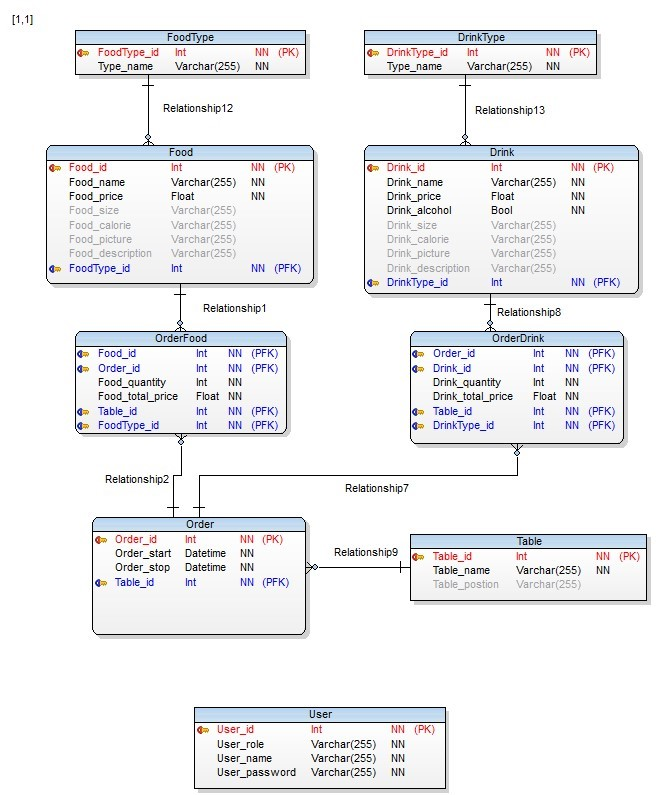
\includegraphics[width=9cm]{Database_physical}
\end{center}
\caption{Končna podatkovna baza za aplikacijo}
\label{Database_physical}
\end{figure}

Končne različice podatkovne baze nisem naredil v prvem poskusu, npr. prvič sem pozabil na tabeli FoodType in DrinkType, kateri mi zelo poenostavijo delo pri selektivnem prikazovanju pijač in jedi v aplikaciji. 

Po končanem urejanju fizične sheme sem naredil izvoz v MySQL 5.0 kodo, ki sem jo potem uvozil v spletni vmesnik phpMyAdmin. Uvoz ni nič posebnega, kreiral sem podatkovna baza in njeno ime ter naredil uvoz. 
Ko je bila podatkovna baza uvožena sem jo potreboval samo še napolniti s podatki. Zadeve sem se prav tako lotil preko phpMyAdmin vmesnika, ki je zelo enostaven in omogoča dodajanje več podatkov na enkrat. Podatke sem črpal iz znanih slovenskih aplikacij za naročanje hrane na dom, eHrana in Wolt.
\begin{figure}[h]
\begin{center}
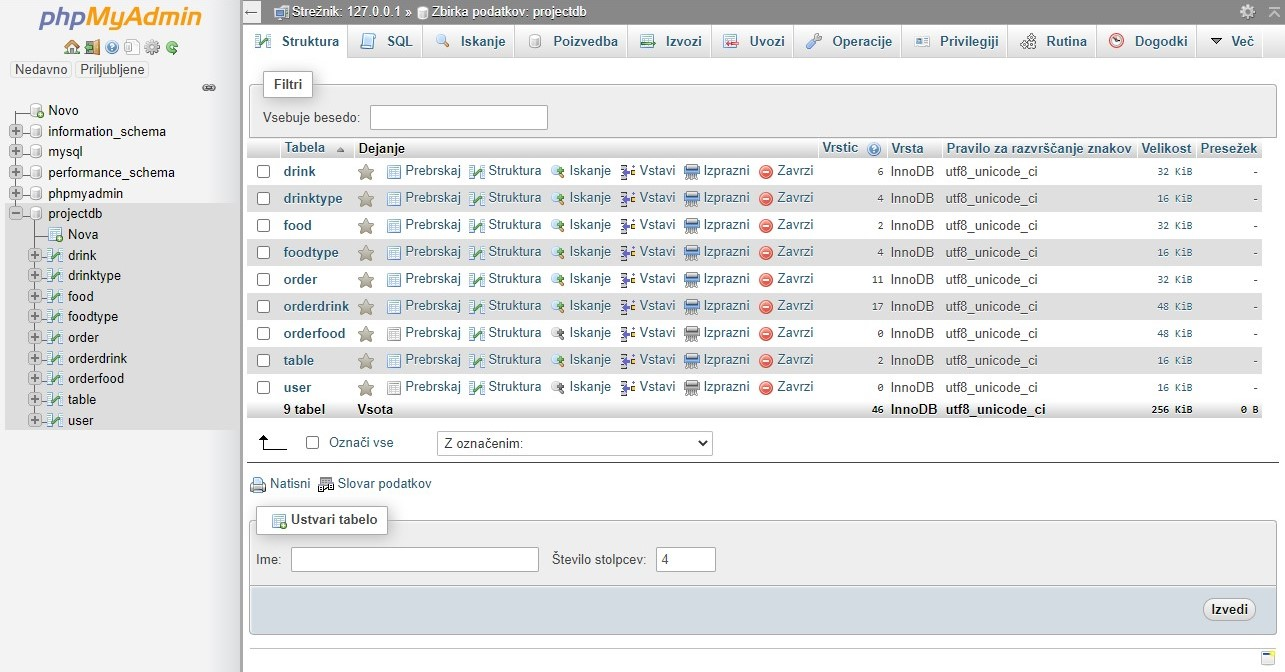
\includegraphics[width=14cm]{phpMyAdmin}
\end{center}
\caption{Izgled podatkovne baze v aplikaciji phpMyAdmin}
\label{phpMyAdmin}
\end{figure}

\section{Strežnik}

\section{Aplikacija}

\chapter {Delovanje aplikacije}
\section{Vmesnik za gost}
\section{Vmesnik za natakarja}
\section{Vmesnik za kuharja}
\section{Primeri uporabe}

\chapter {Sklepne ugotovitve}
\newpage %dodaj po potrebi, da bo številka strani za Literaturo v Kazalu pravilna!
\ \\
\clearpage
\addcontentsline{toc}{chapter}{Literatura}
\bibliographystyle{plain}
\bibliography{literatura}


\end{document}

